% 独立训练固定模型；校准秩构造阈值，不把图示当作覆盖检验。
\begin{tikzpicture}[figure picture,foundation picture,
 trust step/.style={draw=FigureStroke,line width=.7pt,rounded corners=1.5pt,minimum width=36mm,minimum height=20mm,align=center,inner sep=1.5mm}]
 \path[use as bounding box] (0,-9) rectangle (163.2,74);
 \node[trust step,fill=MutedGreenFill] (train) at (18,61) {独立训练\\固定模型$f$};
 \node[trust step,fill=FigureBlueFill] (cal) at (60,61) {校准$n=9,\alpha=0.2$\\$s_i=|y_i-f(\bm x_i)|$};
 \node[trust step,fill=FigureRedFill] (rank) at (102,61) {排序取阈值\\$k=8,\ q=s_{(8)}=0.8$};
 \node[trust step,fill=MutedGreenFill,minimum width=38mm] (test) at (144,61) {新输入$\bm x$\\构造区间$C(\bm x)$};
 \draw[foundation flow] (train.east)--(cal.west);
 \draw[foundation flow] (cal.east)--(rank.west);
 \draw[foundation flow] (rank.east)--(test.west);
 \node[inner sep=0pt] at (53,26) {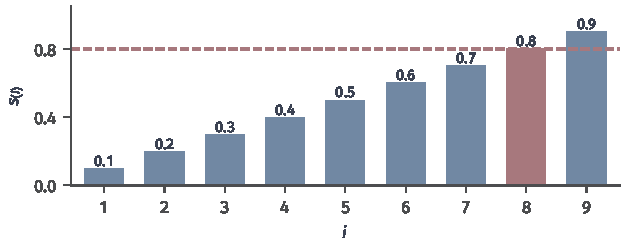
\includegraphics[width=106mm]{figures/02-foundations/03-trustworthiness/tikz/trust-conformal-construction/trust-conformal-construction.pdf}};
 \node[foundation note] at (134,41) {中心$f(\bm x)$，半宽$q$};
 \draw[draw=FigureStroke,line width=.6pt] (112,23)--(158,23);
 \draw[draw=LancetGreen,line width=1.5pt] (116,23)--(154,23);
 \foreach \x in {116,135,154}{\draw[draw=FigureStroke,line width=.7pt] (\x,20)--(\x,26);}
 \node[foundation note,anchor=north] at (116,18) {$f(\bm x)-q$};
 \node[foundation note,anchor=north] at (135,18) {$f(\bm x)$};
 \node[foundation note,anchor=north] at (154,18) {$f(\bm x)+q$};
 \node[foundation note] at (134,0) {$C(\bm x)=[f(\bm x)-q,f(\bm x)+q]$};
\end{tikzpicture}
